\documentclass[a4paper,titlepage,11pt,twosides,floatssmall]{mwrep}
\usepackage[left=2.5cm,right=2.5cm,top=2.5cm,bottom=2.5cm]{geometry}
\usepackage[OT1]{fontenc}
\usepackage{polski}
\usepackage{amsmath}
\usepackage{amsfonts}
\usepackage{amssymb}
\usepackage{graphicx}
\usepackage{url}
\usepackage{tikz}
\usetikzlibrary{arrows,calc,decorations.markings,math,arrows.meta}
\usepackage{rotating}
\usepackage[percent]{overpic}
\usepackage[utf8]{inputenc}
\usepackage{xcolor}
\usepackage{pgfplots}
\usetikzlibrary{pgfplots.groupplots}
\usepackage{listings}
\usepackage{matlab-prettifier}
\usepackage{siunitx}
\definecolor{szary}{rgb}{0.95,0.95,0.95}
\sisetup{detect-weight,exponent-product=\cdot,output-decimal-marker={,},per-mode=symbol,binary-units=true,range-phrase={-},range-units=single}

%konfiguracje pakietu listings
\lstset{
	backgroundcolor=\color{szary},
	frame=single,
	breaklines=true,
}
\lstdefinestyle{customlatex}{
	basicstyle=\footnotesize\ttfamily,
	%basicstyle=\small\ttfamily,
}
\lstdefinestyle{customc}{
	breaklines=true,
	frame=tb,
	language=C,
	xleftmargin=0pt,
	showstringspaces=false,
	basicstyle=\small\ttfamily,
	keywordstyle=\bfseries\color{green!40!black},
	commentstyle=\itshape\color{purple!40!black},
	identifierstyle=\color{blue},
	stringstyle=\color{orange},
}
\lstdefinestyle{custommatlab}{
	captionpos=t,
	breaklines=true,
	frame=tb,
	xleftmargin=0pt,
	language=matlab,
	showstringspaces=false,
	%basicstyle=\footnotesize\ttfamily,
	basicstyle=\scriptsize\ttfamily,
	keywordstyle=\bfseries\color{green!40!black},
	commentstyle=\itshape\color{purple!40!black},
	identifierstyle=\color{blue},
	stringstyle=\color{orange},
}

%wymiar tekstu (bez �ywej paginy)
\textwidth 160mm \textheight 247mm

%ustawienia pakietu pgfplots
\pgfplotsset{
tick label style={font=\scriptsize},
label style={font=\small},
legend style={font=\small},
title style={font=\small}
}

\def\figurename{Rys.}
\def\tablename{Tab.}

%konfiguracja liczby p�ywaj�cych element�w
\setcounter{topnumber}{0}%2
\setcounter{bottomnumber}{3}%1
\setcounter{totalnumber}{5}%3
\renewcommand{\textfraction}{0.01}%0.2
\renewcommand{\topfraction}{0.95}%0.7
\renewcommand{\bottomfraction}{0.95}%0.3
\renewcommand{\floatpagefraction}{0.35}%0.5

\begin{document}
\frenchspacing
\pagestyle{uheadings}

%strona tytu�owa
\title{\bf Sprawozdanie z projektu nr 2, zadanie nr 11\vskip 0.1cm}
\author{Kamil Gabryjelski, Paweł Rybak, Paweł Walczak}
\date{2017}

\makeatletter
\renewcommand{\maketitle}{\begin{titlepage}
\begin{center}{\LARGE {\bf
Wydział Elektroniki i Technik Informacyjnych}}\\
\vspace{0.4cm}
{\LARGE {\bf Politechnika Warszawska}}\\
\vspace{0.3cm}
\end{center}
\vspace{5cm}
\begin{center}
{\bf \LARGE Projektowanie układów sterowania\\ (projekt grupowy) \vskip 0.1cm}
\end{center}
\vspace{1cm}
\begin{center}
{\bf \LARGE \@title}
\end{center}
\vspace{2cm}
\begin{center}
{\bf \Large \@author \par}
\end{center}
\vspace*{\stretch{6}}
\begin{center}
\bf{\large{Warszawa, \@date\vskip 0.1cm}}
\end{center}
\end{titlepage}
}
\makeatother

\maketitle

\tableofcontents
\chapter{Opis obiektu}
\label{sec:opis}
Obiekt używany w projekcie jest symulacją obiektu, napisaną w języku MATLAB.
Opisywany jest on wzorem
\begin{equation}
  Y(k) = f(U(k - 7), U(k - 8), Z(k - 3), Z(k - 4), Y(k - 1), Y(k - 2))
\end{equation}
gdzie $k$ jest aktualną chwilą symulacji.
Wartości sygnałów w punkcie pracy mają wartość $u=y=z=0$. Okres próbkowania wynosi $T_p=0,5s$.
\chapter{Zadanie 1}
\section{Sprawdzenie połączenia}
Zadanie pierwsze polegało na sprawdzeniu możliwości komunikacji ze stanowiskiem.
Sprawdziliśmy to, modyfikując wybrane wejścia obiektu, oraz obserwując zmiany
na obiekcie. Przy modyfikacji wejścia wiatraków widać i słychać było, iż wiatraki kręcą
się wolniej lub szybciej, w zależności od wejścia. Przy sprawdzeniu działania
grzałki polegaliśmy na diodach elektroluminescencyjnych, które świeciły mocniej
lub słabiej w zależności od mocy grzania odpowiedniej grzałki. Nasza pewność
w tej sprawie jest oparta na zaufaniu do konstruktora obiektu. Możliwość
pomiaru wyjśc obiektu zoastała sprawdzona w oparciu o trendy pomiaru,
w zależności od wysterowania wcześniej wspomnianych wejść. Otóż, przy
zwiększeniu mocy grzałki lub zmniejszeniu mocy wiatraka temperatura
na czujniku bliższym danej grzałce i wiatrakowi rośnie szybko, a na dalszym
rośnie wolniej. Przy zwiększaniu mocy wiatraka lub zmniejszaniu mocy grzałki pomiar
temperatur spadał. Podobnie jak wcześniej działo się to z szybkością odwrotnie proporcjonalną
do odległości czujnika od wiatraka i grzałki których sterowanie jest zmieniane.
\section{Punkt pracy}
Punkt pracy naszego stanowiska wynosił $G1 = 27$, $G2 = 32$, $W1 = 50$, $W2 = 50$.
Przy tak ustawionych wejściach pozwoliliśmy obiektowi się ustabilizować. Z powodów
różnych zakłóćeń pomiary temperatury nieustannie się wahały. Oszacowaliśmy
arbitralnie iż, pomiary ustabilizowały się na wartościach $T1 = 35$, $T2 = 36.68$.
Pomiary wyjść przy takich ustawieniach sygnałów wejściowych przedstawia wykres
\ref{fig:pkt_pracy}.

\begin{figure}[tb]
\centering
\begin{tikzpicture}
\begin{axis}[
width=0.75\textwidth,
height = 0.6\textwidth,
xmin=0,xmax=150,ymin=32.5,ymax=37,
xlabel={czas [s]},
ylabel={temperatura [$^\circ$C]},
xtick={0, 50, 100, 150},
ytick={32.5, 33, 33.5, 34, 34.5, 35, 35.5, 36, 36.5, 37},
legend pos=south east,
/pgf/number format/.cd,
use comma,
1000 sep={}
]

\addplot[blue,semithick] file {wykresy/pkt_pracy_y1.txt};
\addplot[red,semithick] file {wykresy/pkt_pracy_y2.txt};
\legend{Temperatura T1, Temperatura T2}

\end{axis}
\end{tikzpicture}
\caption{Punkt pracy obiektu.}
\label{fig:pkt_pracy}
\end{figure}

\chapter{Badanie zachowania obiektu}
\label{sec:zad2}
\section{Odpowiedzi skokowe}
Aby lepiej poznać naturę obiektu przeprowadzone zostały ogólne badania
zachowania obiektu i jego odpowiedzi na różne skoki wartości sterującej.
Eksperyment zakładał, iż na początku obiekt będzie w punkcie pracy
($Y = 0$, $U = 0$), a następnie, w chwili $k = 7$ wykonany zostanie skok do zaplanowanej wcześniej wartości sterowania. Biorąc pod uwagę ograniczenia na wartość sterowania $U^{min} = -1$ i $U^{max} = 1$ wartość sterowania
po skoku mieściła się w owym zakresie. Wyniki eksperymentu zostały zobrazowane
na wykresie \ref{fig:skoki}.


\begin{figure}[tb]
\centering
\begin{tikzpicture}
\begin{axis}[
width=0.75\textwidth,
xmin=0,xmax=200,ymin=-0.5,ymax=4.5,
xlabel={Chwila (k)},
ylabel={Wyjście (y)},
legend pos=north east,
/pgf/number format/.cd,
use comma,
1000 sep={},
cycle list name=color
]
\addplot file {wykresy/zad2_y_1.txt};
\addplot file {wykresy/zad2_y_2.txt};
\addplot file {wykresy/zad2_y_3.txt};
\addplot file {wykresy/zad2_y_4.txt};
\addplot file {wykresy/zad2_y_5.txt};
\addplot file {wykresy/zad2_y_6.txt};
\addplot file {wykresy/zad2_y_7.txt};
\addplot file {wykresy/zad2_y_8.txt};
\addplot file {wykresy/zad2_y_9.txt};
\addplot file {wykresy/zad2_y_10.txt};
\legend{$U = -1$,$U = -0.8$,$U = -0.6$,$U = -0.4$,$U = -0.2$,$U = 0.2$,
		$U = 0.4$, $U = 0.6$, $U = 0.8$, $U = 1$}
\end{axis}
\end{tikzpicture}
\caption{Odpowiedzi skokowe dla różnych wartości sterowania.
(Wartość końcowa sterowania w legendzie)}
\label{fig:skoki}
\end{figure}

\section{Charakterystyka statyczna}
Następnie wyznaczona została charakterystyka statyczna obiektu. Znaleziona
została poprzez sprawdzenie przy jakiej wartości wyjścia obiekt stabilizuje
się dla danej wartości sterowania. Na podstawie tego sporządzony został wykres.
Wyniki zostały zamieszczone na wykresie \ref{fig:char_stat}.
\begin{figure}[H]
\centering
\begin{tikzpicture}
\begin{axis}[
width=0.75\textwidth,
xmin=-1,xmax=1,ymin=-0.5,ymax=5,
xlabel={Sterowanie (u)},
ylabel={Wyjście (y)},
/pgf/number format/.cd,
use comma,
1000 sep={}
]
\addplot file {wykresy/zad2_yu.txt};
\end{axis}
\end{tikzpicture}
\caption{Charakterystyka statyczna obiektu.}
\label{fig:char_stat}
\end{figure}

Otrzymana charakterystyka przedstawiona na wykresie \ref{fig:char_stat} jest nieliniowa. Nie można zatem określić wzmocnienia statycznego. Ponadto należy się spodziewać, że "tradycyjne" regulatory PID i DMC, przystosowane do obiektów liniowych, mogą mieć problemy z prawidłową regulacją.


\section{Charakterystyka dynamiczna}
Charakterystyka dynamiczna obiektu wyznaczana jest na podstawie czasu potrzebnego na osiągnięcie co najmniej $90\%$ wartości końcowej wyjścia. Oś odciętych stanowią wartości sterowania, zaś na osi rzędnych wykresu znajdują się chwile $k$, w których zostało osiągnięte $90\%$ wartości końcowej wyjścia. Wynik eksperymentu przedstawia wykres \ref{fig:char_dyn}.
\begin{figure}[H]
\centering
\begin{tikzpicture}
\begin{axis}[
width=0.75\textwidth,
xmin=-1,xmax=1,ymin=14,ymax=26,
xlabel={$U$},
ylabel={chwila $k$},
/pgf/number format/.cd,
use comma,
1000 sep={}
]
\addplot file {wykresy/zad2_kd.txt};
\end{axis}
\end{tikzpicture}
\caption{Charakterystyka dynamiczna obiektu.}
\label{fig:char_dyn}
\end{figure}

Jak widać na wykresie \ref{fig:char_dyn}, charakterystyka dynamiczna obiektu nie jest liniowa.
\chapter{Zadanie 3}
Celem zadania trzeciego było przeksztalcenie jednej z otrzymanych odpowiedzi skokowych używając w tym celu
członu inercyjnego drugiego rzędu z opóźnieniem. Wzór ogólny takiego obiektu przedstawia równanie \ref{eq:2in_op}.
\begin{equation}
  \label{eq:2in_op}
  y(k) = b_1u(k-T_D-1) + b_2u(k-T_D-2)-a_1y(k-1)-a_2y(k-2),
\end{equation}
gdzie
\begin{align}
  a_1 &= -e^{-\frac{1}{T_1}}-e^{-\frac{1}{T_2}} \nonumber \\
  a_2 &= e^{-\frac{1}{T_1}}e^{-\frac{1}{T_2}} \nonumber \\
  b_1 &= \frac{K}{T_1 - T_2}[T_1(1 - e^{-\frac{1}{T_1}}) - T_2(1 - e^{-\frac{1}{T_2}})] \nonumber \\
  b_2 &= \frac{K}{T_1 - T_2}[e^{-\frac{1}{T_1}}T_2(1 - e^{-\frac{1}{T_2}}) - e^{-\frac{1}{T_2}}T_1(1 - e^{-\frac{1}{T_1}})]
\end{align}
Przybliżenie polega na takim dobraniu parametrów $T_1$, $T_2$, $K$, oraz $T_D$ tak,
aby różnica między faktycznym wyjściem obiektu i przybliżeniem była jak najmniejsza.
Do doboru parametrów użyliśmy funkcji \texttt{GA}.  Do znormalizowania wykorzysaliśmy odpowiedź
skokową, gdzie skok sterowania wynosił $\Delta U = 13$ (do wartości sterowania $U = 40$). Nasz wybór
motywujemy, tym że otrzymana odpowiedź była najmniej zaszumiona. Procesu normalizacji odpowiedzi skokowej, przed poddaniem
jej aproksymacji, nie będziemy tutaj opisywać, ze względu na dokładny opis owego procesu
w poprzednich sprawozdaniach.
% Ciężko jest szacować wspomniane wartości same w sobie. Mając jednak wiedzę, że wynikają
% one z innych parametrów charakterystycznych dla członu dwuinercyjnego z opóźnieniem,
% można już próbować je szacować. Owe zależności wyglądają następująco:
% Jako wartości początkowe parametrów $T_1$, $T_2$, $K$, oraz $T_D$ wybraliśmy odpowiednio
% 5, 10, 2, oraz 9. Wybralismy 2 dla K (zebrane odpowiedzi nie wskazywały dużego wzmocnienia),
% TD = 9 (na tyle oceniamy opóźnienie obiektu), oraz T1 i T2  jako 5 i 10 (wartości z grubsza losowe).
%PIERDOLENIE
Do przybliżenia użyliśmy algorytm ewolucyjny, który nie używa punktu początkowego,
a losowej populacji początkowej. Dlatego jedyne parametry algorytmu to ogarniczenia
Kierując się logiką ograniczyliśmy od dołu parametry zerami, zaś od góry wartościami 1000, 1000, 10, 50,
dla zmiennych odpowiednio $T_1$, $T_2$, $K$, oraz $T_D$.
Aproksymacja odpowiedzi skokowej została pokazana na rysunku \ref{fig:approx}.

\begin{figure}[tb]
\centering
\begin{tikzpicture}
\begin{axis}[
width=0.75\textwidth,
height = 0.6\textwidth,
xmin=0,xmax=400,ymin=0,ymax=0.45,
xlabel={$k$},
ylabel={$y$},
xtick={0, 50, 100, 150, 200, 250, 300, 350, 400},
ytick={0, 0.05, 0.1, 0.15, 0.2, 0.25, 0.3, 0.35, 0.4, 0.45},
legend pos=north west,
/pgf/number format/.cd,
use comma,
1000 sep={}
]

\addplot[blue,semithick] file {wykresy/skok40_norm.txt};
\addplot[red,semithick] file {wykresy/skok40_approx.txt};
\legend{Odpowiedź obiektu, Aproksymacja}

\end{axis}
\end{tikzpicture}
\caption{Aproksymacja odpowiedzi skokowej obiektu.}
\label{fig:approx}
\end{figure}

%\chapter{chapter name}

Eksperymentalne testy w poszukiwaniu lepszy nastaw regulatora PID rozpoczynamy od tych wyznaczonych za pomocą eksperymentu ZN.
Najpierw zaczniemy regulować nastawę Td. Po kilku testach zauważamy spadek błędu, dla wartości Ti = 20. Poprawę oceniamy za pomocą wskaźnika numerycznego Error,
gdyż ciężko jest ujrzeć zmianę obserwując jedynie przebiegi. Następnie sprawdzamy wartość Td. Po testach uważamy za dobrą wartość Td = 4.

%% /******** Optymalizacja *********/
\chapter{Optymalizacja}
Do wyznaczenia optymalnych parametrów regulatorów PID i DMC użyliśmy funkcji \emph{fmincon} oraz \emph{GA}. Są to funkcje pozwalające wyznaczyć minimum (globalne) zadanej funkcji celu.
W obu przypadkach regulatorów, funkcję celu traktujemy jako suma kwadratów błędów ( między wyjściem obiektu a wartością zadaną ).
Do wyznaczenia optymalnych parametrów regulatora PID użyliśmy funkcji \emph{fmincon}. Optymalizujemy trzy parametry: K (wzmocnienie - X(1)), Ti (X(2)) oraz Td (X(3)).
Ograniczeniem jakie przyjmujemy są dodatnie wartości parametrów regulatora. Po uruchomieniu \emph{fmincon} otrzymujemy następujące parametry:
\begin{align}
  K &= 1.2958 \nonumber \\
  T_d &= 21.8912 \\
  T_i &= 4.7082 \nonumber
\end{align}
Wyniki zostały zobrazowane na wykresie \ref{fig:optim_pid}.
Zauważamy, że funkcja celu przyjmuje niższą wartość niż dla parametrów regulatora wyznaczonego metodą inżynierską, co sugeruje prawidłowe działanie funkcji optymalizacji.
\begin{figure}
  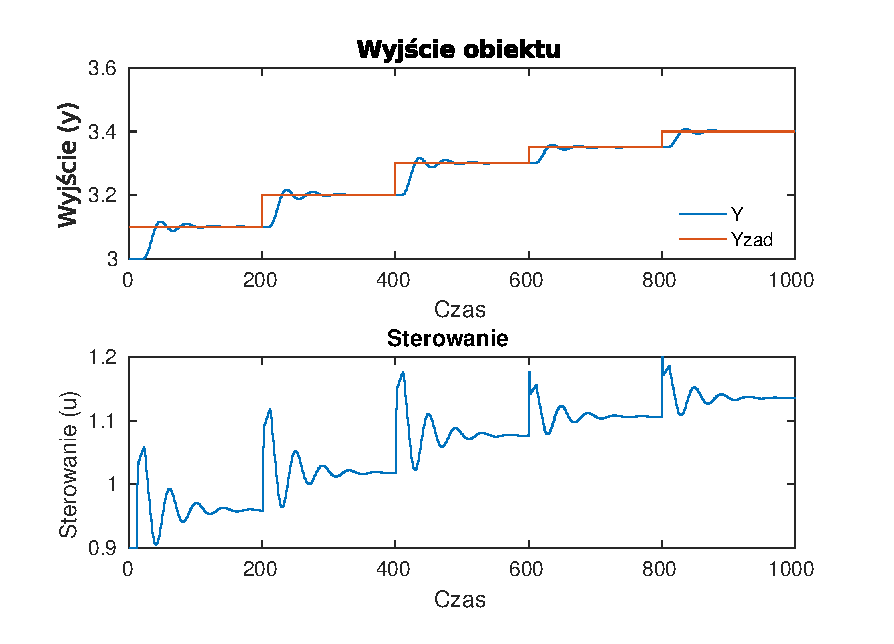
\includegraphics{wykresy/optim_pid.eps}
  \caption{Regulator PID z nastawami wyznaczonymi funkcją \emph{fmincon}.}
  \label{fig:optim_pid}
\end{figure}
Do wyznaczenia optymalnych parametrów regulatora DMC użyliśmy funkcji \emph{GA}. Jest to algorytm genetyczny umożliwiający znalezienie minimum danej funkcji. Optymalizujemy trzy parametry:
N - horyzont predykcji,
Nu - horyzont sterowania,
$\lambda$ - współczynnik 'kary' za zmiany sterowania.
Użycie algorytmu \emph{GA} motywujemy tym, że w przeciwieństwie do \emph{fmincon}, możemy wprowadzić ograniczenie na N oraz Nu, tak aby ich wartości mogły być dodatnie całkowite.
Po uruchomieniu \emph{GA} otrzymujemy następujące parametry:
\begin{align}
  N &= 74 \nonumber \\
  N_u &= 1 \\
  \lambda &= 30.2824 \nonumber
\end{align}
Wyniki obrazuje wykres \ref{fig:optim_dmc}.
Zauważamy, że funkcja celu przyjmuje niższą wartość niż dla parametrów regulatora DMC wyznaczonego na chybił trafił, oraz zdecydowanie lepsze niż parametry optymalne regulatora PID.
\begin{figure}
  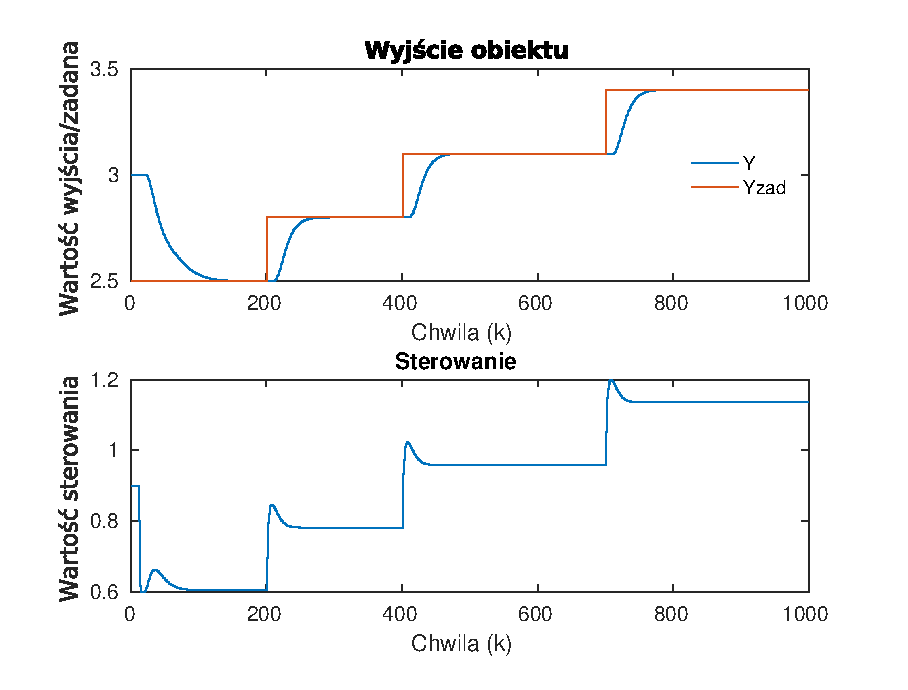
\includegraphics{wykresy/optim_dmc.eps}
  \caption{Regulator DMC z nastawami wyznaczonymi funkcją \emph{GA}.}
  \label{fig:optim_dmc}
\end{figure}

% \input{listingi}
% \input{literatura}
\end{document}
